\documentclass[a4paper,12pt]{report}

\usepackage{alltt, fancyvrb, url}
\usepackage{graphicx}
\usepackage[utf8]{inputenc}
\usepackage{float}
\usepackage{xcolor}
\usepackage{hyperref}

\usepackage[italian]{babel}

\usepackage[italian]{cleveref}

\title{OOP24 - RUNWARRIOR}
\author{
    Samuele Bianchedi, Riccardo Cornacchia\\
    Francesca Gatti, Giovanni Maria Rava}
\date{\today}
\begin{document}
\maketitle
\chapter{Analisi}
\section{Descrizione e requisiti}
Il gruppo si pone come obbiettivo quello di realizzare una reinterpretazione del famoso gioco 
Super Mario Bross del 1986. Il gioco ha come personaggio principale un cavaliere, che tramite 
l'input dell'utente si muove in una mappa 2D. L'obbiettivo del cavaliere è salvare una princessa tenuta
prigioniera da uno stregone, completando diversi livelli che lo condurranno al castello nel quale è 
rinchiusa. Nel gioco sarà possibile, tramite un negozio, comprare un altro personaggio, se si ha raccolto un numero sufficiente di monete.
All'interno del gioco, oltre a diversi ostacoli, sono presenti nemici che il cavaliere può uccidere per rimanere in vita e 
completare il livello. 
\subsection*{Requisiti funzionali}
\begin{itemize}
    \item Il personaggio deve avanzare, indietreggiare e saltare all'interno della mappa.
    \item Gestione delle collisioni del personaggio con nemici, ostacoli, monete e potenziamenti.
    \item Il personaggio può ottenere due potenziamenti che lo aiuteranno nella sua avventura.
    \item Gestione di nemici ed ostacoli diversi in base alla mappa.
    \item Creazione di un sistema di punteggio, che verrà mostrato al completamento del livello.
\end{itemize}
\newpage
\subsection*{Requisiti non funzionali}
\begin{itemize}
    \item Implementazioni di una quarta mappa. 
    \item Gestione di restart e checkpoint.
    \item Creazione di nemici e ostacoli più complessi.
    \item Musica e suoni. 
\end{itemize}
\section{Modello del Dominio}
RunWarrior è gioco ambientato in un mondo fantastico in cui il personaggio principale deve affrontare 3 livelli diversi, selezionabili mediante un menù.
In questi livelli il personaggio deve portersi muovere per sopravvivere e uccidere i nemici. Il movimento del personaggio è gestito tramite tastiera.
All'interno della mappa sono posizionate delle uova che racchiudono al loro interno i 2 possibili powerup, diversi per Warrior e Wizard.
Per il completamento del gioco è neccessario sbloccare tutti i livelli in maniera sequenziale, che si considerano terminati 
tramite l'ingresso in un portale, ad eccezione del terzo che si conclude con il castello della principessa.
All'interno di ogni livello possono essere presenti degli ostacoli letali (MapElement) e dei nemici (Enemy) e delle monete (Coin) con il quale il 
personaggio può collidere. Se ciò accade con un ostacolo o con un nemico perde un potenziamento, nel caso lo avesse, altrimenti la partita finisce.
I nemici sono di 5 tipi:
\begin{itemize}
    \item Goblin
    \item Snake
    \item Wizard
    \item Monkey 
    \item Guard
\end{itemize}
Gli ostacoli letali sono:
\begin{itemize}
    \item Fungo
    \item Cactus
    \item Camino con fuoco
\end{itemize}

\begin{figure}
    \centering
    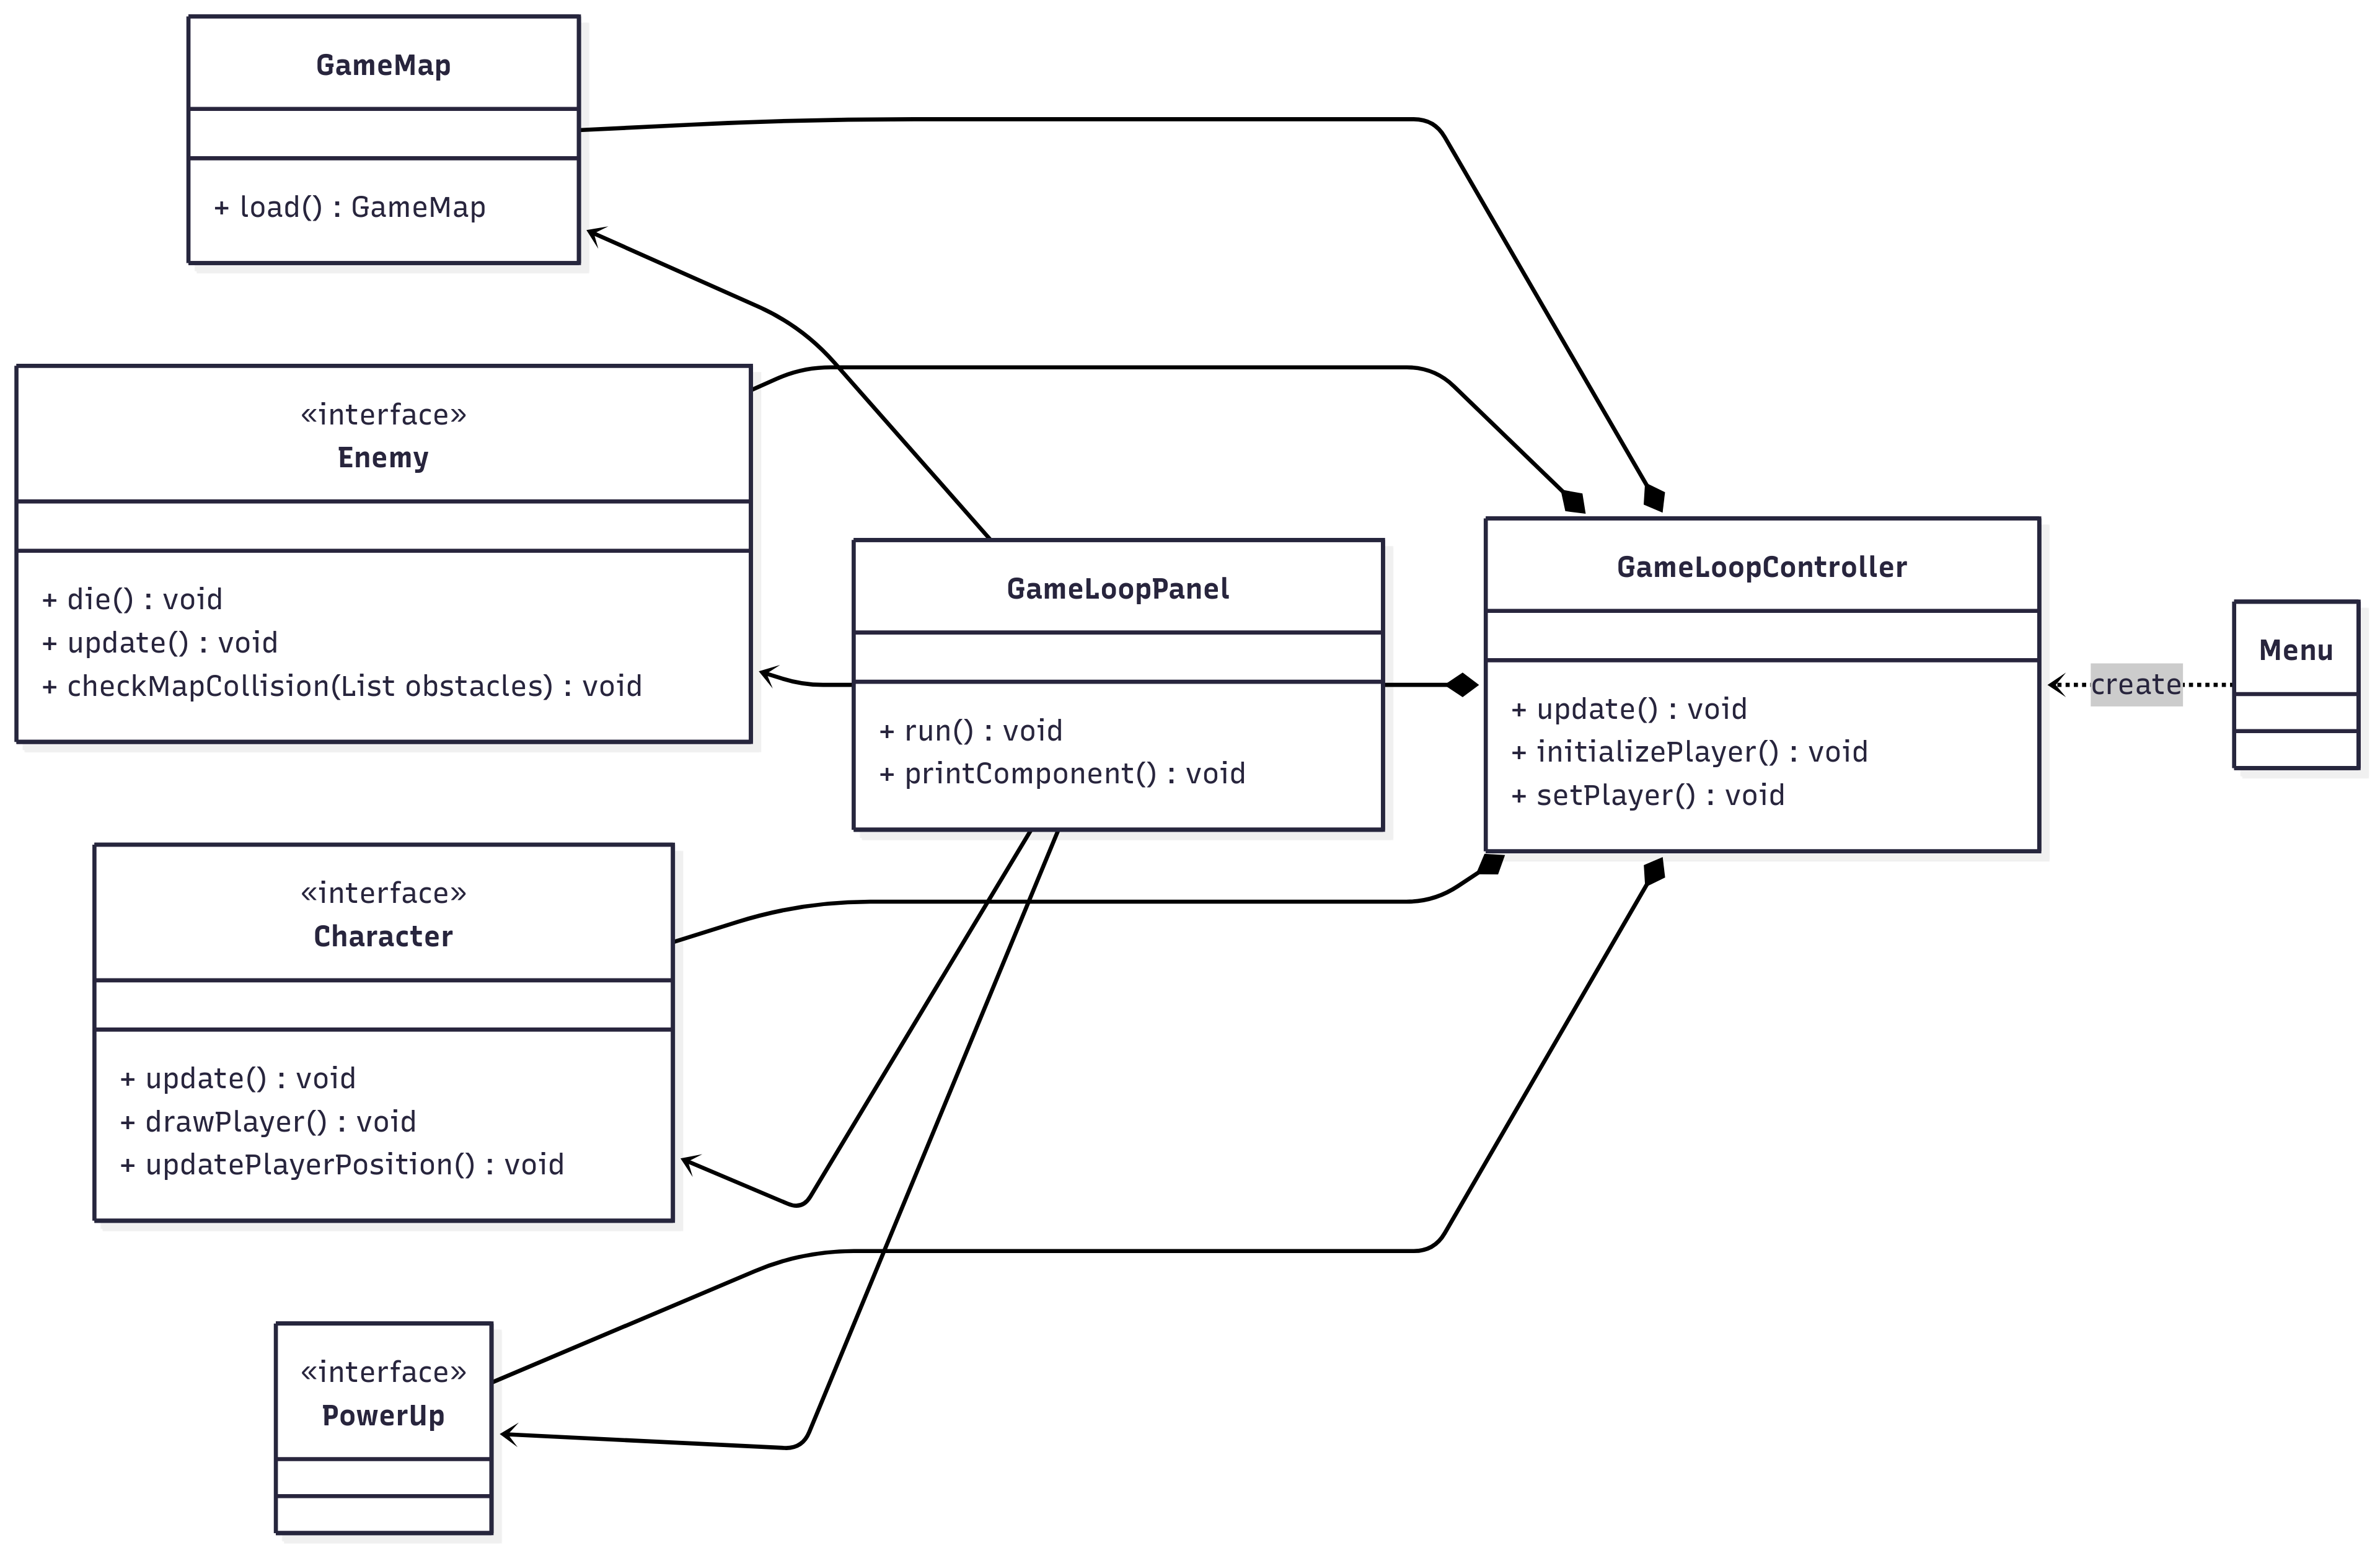
\includegraphics[width=\textwidth]{resources/modelloDominioUML.png}
    \caption{UML del modello del dominio}
    \label{}
\end{figure}
\chapter{Design}
\section{Architettura}
L'architettura di RunWarrior segue il pattern architetturale MVC (Model - View - Controller). Il GameLoopController gestisce l'aggiornamento
del gioco e di tutte le sue entità a seguito dei diversi eventi che possono capitare durante la sessione. All'interno della classe, 
dal momento in cui viene acquistato il nuovo personaggio, ricevendo le informazione da GameSaveManager e Shop, viene gestito il cambio skin.
Gli input da tastiera per muovere il personaggio vengono gestiti tramite la comunicazione tra le classi CharacterComand e MovementHandlerImpl.
Quindi il Character è una entità reattiva che modifica il proprio stato a seguito delle diverse collisioni con le entità, 
tramite CollisionDetection, KillDetection e PowerUpDetection.
Il pattern MVC implementato consente di mantenere lo stato del controller nell'eventualità che si modifichi la view.
inserire UML delle classi principali dell'MVC
\section{Samuele Bianchedi}
\section{Riccardo Cornacchia}
\section{Francesca Gatti}
\section{Giovanni Maria Rava}
\end{document}